% Standalone source of Fig. 1 (compiled to figures/fig_layers.pdf; ieeeaccess.cls clashes with TikZ).
% Build: pdflatex fig_layers_standalone.tex && mv fig_layers_standalone.pdf fig_layers.pdf
\documentclass[border=2pt]{standalone}
\usepackage{mathptmx}
\usepackage{xcolor}
\usepackage{tikz}
\usetikzlibrary{arrows.meta}
\definecolor{authc}{HTML}{EB6834}
\definecolor{payc}{HTML}{2A78D6}
\newcommand{\cpr}{C-PR}
\begin{document}
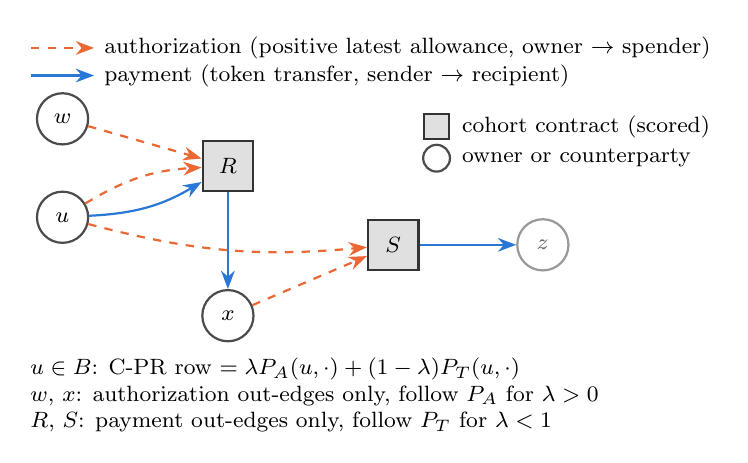
\begin{tikzpicture}[>=Stealth, font=\footnotesize,
  acc/.style={circle, draw=black!70, thick, minimum size=6.5mm, inner sep=0pt, fill=white},
  con/.style={rectangle, draw=black!80, thick, minimum size=6.4mm, inner sep=0pt, fill=black!12},
  auth/.style={->, thick, dashed, draw=authc},
  pay/.style={->, thick, draw=payc}]
  \node[acc] (u)  at (0,0)       {$u$};
  \node[acc] (w)  at (0,1.25)    {$w$};
  \node[acc] (x)  at (2.1,-1.25) {$x$};
  \node[con] (r)  at (2.1,0.65)  {$R$};
  \node[con] (s)  at (4.2,-0.35) {$S$};
  \node[acc, draw=black!40, text=black!60] (z) at (6.1,-0.35) {$z$};
  \draw[auth] (u) to[bend left=14] (r);
  \draw[pay]  (u) to[bend right=14] (r);
  \draw[auth] (u) to[bend right=10] (s);
  \draw[auth] (w) -- (r);
  \draw[auth] (x) -- (s);
  \draw[pay]  (r) -- (x);
  \draw[pay]  (s) -- (z);
  \draw[auth] (-0.4,2.15) -- (0.4,2.15) node[right, text=black] {authorization (positive latest allowance, owner $\to$ spender)};
  \draw[pay] (-0.4,1.8) -- (0.4,1.8) node[right, text=black] {payment (token transfer, sender $\to$ recipient)};
  \node[con, minimum size=3.2mm] at (4.75,1.15) {};
  \node[right] at (4.95,1.15) {cohort contract (scored)};
  \node[acc, minimum size=3.4mm] at (4.75,0.75) {};
  \node[right] at (4.95,0.75) {owner or counterparty};
  \node[align=left, anchor=north west, inner sep=1pt] at (-0.45,-1.75)
    {$u\in B$: \cpr{} row $=\lambda P_A(u,\cdot)+(1-\lambda)P_T(u,\cdot)$\\
     $w$, $x$: authorization out-edges only, follow $P_A$ for $\lambda>0$\\
     $R$, $S$: payment out-edges only, follow $P_T$ for $\lambda<1$};
\end{tikzpicture}
\end{document}
